\documentclass[10pt,journal,compsoc]{IEEEtran}
\IEEEoverridecommandlockouts
% The preceding line is only needed to identify funding in the first footnote. If that is unneeded, please comment it out.
\usepackage{cite}
\usepackage{amsmath,amssymb,amsfonts}
% \usepackage{algorithmic}
\usepackage{graphicx}
\usepackage{textcomp}
\usepackage{xcolor}
\usepackage{subcaption}
\renewcommand\thesubfigure{(\alph{subfigure})}
\captionsetup[sub]{labelformat=simple}

\usepackage{hyperref}
%\renewcommand{\figureautorefname}{Fig.}
\usepackage{mwe}
\usepackage{float}
% \usepackage{amsmath}
\usepackage{caption,tabularx,booktabs}
\usepackage{multirow}


%\usepackage{algorithmic}
\usepackage{booktabs} % For formal tables
\usepackage{array}
%\usepackage{algorithmicx,algorithm}
\usepackage[ruled]{algorithm2e}
\usepackage[noend]{algpseudocode}
\usepackage[capitalise]{cleveref}
\usepackage{caption}
\usepackage{url}
\usepackage{flushend}
\pagenumbering{arabic}
\usepackage{fancyhdr}
\renewcommand{\headrulewidth}{0pt}
\renewcommand{\footrulewidth}{0pt}

\usepackage{array}
\newcommand{\PreserveBackslash}[1]{\let\temp=\\#1\let\\=\temp}
\newcolumntype{C}[1]{>{\PreserveBackslash\centering}p{#1}}
\newcolumntype{R}[1]{>{\PreserveBackslash\raggedleft}p{#1}}
\newcolumntype{L}[1]{>{\PreserveBackslash\raggedright}p{#1}}

\def\BibTeX{{\rm B\kern-.05em{\sc i\kern-.025em b}\kern-.08em
    T\kern-.1667em\lower.7ex\hbox{E}\kern-.125emX}}

\newcommand{\EG}{\textit{e.g.}}
\newcommand{\notes}[1]{\textcolor{red}{***{#1}***}}
\newcommand{\name}{\textit{PUAnomaly}}
\newcommand{\ROCKA}{ROCKA}
\newcommand{\CPLE}{CPLE}
\newcommand{\ETC}{\textit{etc}}

\newcommand{\tabincell}[2]{\begin{tabular}{@{}#1@{}}#2\end{tabular}}%���ڵ�����
\makeatletter
\def\hlinew#1{%
  \noalign{\ifnum0=`}\fi\hrule \@height #1 \futurelet
   \reserved@a\@xhline}
% \definecolor{darkred}{rgb}{0.55, 0.0, 0.0}
\newtheorem{definition}{Definition}

\begin{document}

\title{Rapid and Robust Anomaly Detection for Large Number of KPI Streams
%{\footnotesize \textsuperscript{*}Note: Sub-titles are not captured in Xplore and
%should not be used}
%\thanks{Identify applicable funding agency here. If none, delete this.}
}

\author{\IEEEauthorblockN{Anonymous Author(s)}}
% \author{
% \IEEEauthorblockN{Jiahao Bu\IEEEauthorrefmark{2}\IEEEauthorrefmark{5},
% Ying Liu\IEEEauthorrefmark{2}\IEEEauthorrefmark{5}, 
% Shenglin Zhang\thanks{\IEEEauthorrefmark{1} Shenglin Zhang is the corresponding author.}\IEEEauthorrefmark{3}\IEEEauthorrefmark{1},
% Weibin Meng\IEEEauthorrefmark{2}\IEEEauthorrefmark{5},
% Qitong Liu\IEEEauthorrefmark{4},
% Xiaotian Zhu\IEEEauthorrefmark{4},
% Dan Pei\IEEEauthorrefmark{2}\IEEEauthorrefmark{5}}
% Dan Pei\thanks{\IEEEauthorrefmark{1} Dan Pei is the corresponding author.}\IEEEauthorrefmark{2}\IEEEauthorrefmark{5}\IEEEauthorrefmark{1}}

% \IEEEauthorblockA{\IEEEauthorrefmark{2}Tsinghua University   
% \IEEEauthorrefmark{3}Nankai University   
% \IEEEauthorrefmark{4}Tencent} 
% \IEEEauthorblockA{\IEEEauthorrefmark{5}Beijing National Research Center for Information Science and Technology (BNRist)  } 
% Email: bjh16@mails.tsinghua.edu.cn, liuying@cernet.edu.cn, zhangsl@nankai.edu.cn, mwb16@mails.tsinghua.edu.cn
% \\  \{cloudliu, markxtzhu\}@tencent.com, peidan@tsinghua.edu.cn
% }


\maketitle
	% \thispagestyle{plain}
	% \pagestyle{plain}
	\thispagestyle{fancy}
	\fancyhead{} 
	\lhead{} 
% 	\lfoot{978-1-5386-6808-5/18/\$31.00 \copyright2018 IEEE}
	\cfoot{} 
	\rfoot{}

%!TEX root = ../cluster_semi.tex
\begin{abstract}
To ensure the reliability of software applications and systems, Internet-based services monitor and detect anomalies for their KPI streams (Key Performance Indicator, such as CPU utilization, number of queries per second, response latency). %However,
Neither unsupervised nor supervised learning methods meet the requirements of anomaly detection because of the large number of KPI streams and the lack of labels. Semi-supervised learning methods ensure the accuracy of anomaly detection with reducing the manual labeling effort, however, all samples in specific time series  segments need to be carefully labeled.
In this paper, we propose \name{}, which integrates both PU learning and active learning techniques.
% PU learning enables us to train an anomaly detection model by only randomly labeling a few anomalies of several typical historical/existing KPI streams.
PU learning allows us to train an anomaly detection model only by randomly labeling a small number of anomalies in a few typical historical/existing KPI streams.
Active learning is applied to select the most reliable samples for manual labeling in the iterations of PU learning.
%Through experiments,we show that
\name{} achieves the best F-score over 0.83 on 80 new KPI streams, almost as the same as a state-of-the-art supervised approach, greatly outperforming a state-of-the-art unsupervised approach. Compared with the semi-supervised method, the bset F-score of \name{} is about 0.19 higher than the semi-supervised.

\end{abstract}
%!TEX root = ../cluster_semi.tex
\section{Introduction}
\label{sec:introduction}
% To ensure the stability of the service, large Internet companies need to closely monitor sundry KPIs(Key Performance Indicators, \EG{}, Page Views, success rate, number of online users and latency) to detect anomaly points as soon as possible. T
% he anomaly points on KPIs are data patterns that have different data characteristics from normal(\EG{}, jitters, slow ramp-ups, spikes or dips). 
% They often indicate potential risks of related services(\EG{}, machine malfunction, cyber attacks and network overload)~\cite{chen2013provider,zhang2015rapid}. 
% The detection of anomaly points can reduce the loss of the enterprise. So accurate anomaly detection technology is especially critical.

% \notes{zihan}
Internet-based services (\EG, online games, online shopping, social networks, search engine) monitor 
% thousands to millions of
 \textit{KPIs} (\textit{Key Performance Indicators}, say CPU utilization, number of queries per second, response latency) of  their applications and systems in order to keep their services reliable.  
Anomalies on KPI (\EG, a spike or dip in a KPI stream) likely indicate underlying failures on Internet services~\cite{chen2013provider,liu2015opprentice,zhang2015rapid,ma2018robust,sun2018hotspot}, such as server failures, network overload, external attacks, and should be accurately and rapidly detected. 


Despite the rich body of literature in KPI anomaly detection~\cite{Mahimkar:2011:RDM:2079296.2079309, barford2002signal, Zhang:2005:NA:1251086.1251116, yan2012argus, egads, liu2015opprentice, ding2013anomaly, xu2018unsupervised}, there remains one common and important scenario that has not been studied or well-handled by any of these approaches. Specifically, when large number of KPI streams emerge \emph{continuously and frequently}, operators need to deploy accurate anomaly detection models for these new KPI streams as quickly as possible (\textit{e.g.}, within 3 weeks at most), in order to avoid that Internet-based services suffer from false alarms (due to low precision) and/or missed alarms (because of low recall) and in turn impact on user experience and revenue. Large number of new KPI streams emerge due to the following two reasons. First, new products can be frequently launched, such as in gaming platform. For example, in a top gaming company $G$ studied in this paper, on average over ten new games are launched per quarter, which results in more than 6000 new KPI streams per 10 days on average. Second, with the popularity of DevOps and micro-service, software upgrades become more and more frequent~\cite{zhang2016funnel}, many of which result in the pattern changes of existing KPI streams, making the previous anomaly detection algorithms/parameters outdated. 

	
Unfortunately, none of the existing anomaly detection approaches, including \emph{traditional statistical algorithms, supervised learning, and unsupervised learning}, are feasible to deal with the above scenario well. 
For \emph{traditional statistical algorithms}~\cite{Mahimkar:2011:RDM:2079296.2079309, barford2002signal, Zhang:2005:NA:1251086.1251116, yan2012argus}, to achieve the best accuracy, operators have to manually select an anomaly detection algorithm and tune its parameters for \emph{each KPI stream}, which is infeasible for the large number of emerging KPI streams. \emph{Supervised learning} based methods~\cite{egads, liu2015opprentice} require manually labeling anomalies for each new KPI stream, which is not feasible for the large number of emerging KPI streams either. \emph{Unsupervised learning} based methods~\cite{ding2013anomaly, xu2018unsupervised} do not require algorithm selection, parameter tuning, or manual labels, but they either suffer from low accuracy~\cite{zhang2018anomaly} or require large amounts of training data for each new KPI stream (\textit{e.g.}, six months worth of data)~\cite{xu2018unsupervised}, which do not satisfy the requirement of rapid deployment (\textit{e.g.}, within 3 weeks) of accurate anomaly detection.
% take all anomaly scores calculated by traditional statistical algorithms as features to train models

% With the labelled data, supervised learning  methods are explored. Different from majority vote, these methods can learn the importance of statistical algorithms from data, thereby give the prediction. EGA,,DS~\cite{egads}, and Opprentice~\cite{liu2015opprentice} use label information which experienced operators give according to their domain knowledge to achieve better performance. But these methods heavily rely on precise label. Experts can not label anomaly for every KPI stream. Once a new game launch, experts need to give label for these new KPI streams, which is not feasible.

% \textbf{Unsupervised learning based methods.} To solve algorithm selection and parameter tuning problem, unsupervised learning based methods are explored. These methods take all anomaly scores calculated by above traditional statistical algorithms as features to train models. To name some representative, One-class SVM~\cite{perdisci2006using}, isolation based methods~\cite{liu2012isolation}, and so on. Unsupervised methods are used widely in practice because they do not need experts to label data. However, these method's performance do not always achieve what company expected. 

% \textbf{Supervised learning based methods.} 
% Operators have to 
% In practice, experts need to choose effective algorithms and fine-tune algorithm's parameters for different type KPIs. 
% Obviously, these algorithms are limited and cannot be used in large number of KPIs.



% However, most anomaly detection algorithms (\EG, Opprentice~\cite{liu2015opprentice}, EDAGS~\cite{egads}, DONUT~\cite{xu2018unsupervised}) assume that an individual model is needed for each KPI. Thus, large-scale anomaly detection on thousands to millions of KPIs is very challenging due to the large overhead of model selection, parameter tuning, model training, or anomaly labeling. 
% Fortunately, many KPIs are similar due to their implicit associations  and similarities. If we can identify homogeneous KPIs (\EG, number of queries per server in a well-loaded balanced server cluster) based on their similarities and group them into a few clusters, perhaps only one anomaly detection model is needed per cluster, thus significantly reducing the various overhead aforementioned.

% A real world application KPI is a time series with a stable time interval collected by the surveillance system.
% In this paper, we focus on game-related KPIs. Compared to other fields, game-related KPIs have some unique characteristics.
% \begin{itemize}
% 	\item The amount is exceedingly huge. A famous game company always operates hundreds of games simultaneously and monitors millions of KPIs (\EG{} success rate, the number of online gamers and latency). Anomaly detection on so large scale KPIs is an enormous challenge.
% 	\item The new KPIs will continue to emerge. Only tiny amounts of games can run stably. The new games will replace the games which have short lifes span continuously. With the on-line launch of new games, new KPIs should also be monitored immediately. These is the large overhead of algorithms selection and anomaly labeling.
% \end{itemize}
% Different from other service's KPIs, the game-related KPIs are always numerous. In addtion, the new KPIs will continue to emerge with the operation of new games. 
% Over the years, some traditional time series algorithm~\cite{knorn2008adaptive, lu2009network, pincombe2005anomaly, chen2013provider, yan2012argus} are uesd for KPI anomaly detection. But, they suffer from the overhead of algorithm picking and parameter tuning. In the field of machine learning, unsupervised learning based methods~\cite{perdisci2006using, liu2012isolation} can't always get satisfying performance. Supervised learning based methods perform well enough, but heavily rely on precise labels. The experts can't label anomaly points for every new KPIs.

% Over the years, a large number of anomaly detection algorithms or systems for KPIs have appeared. However, most of them are designed for only a single KPI and can't be applied for millions of KPIs in our scenario. They suffer from the overhead of algorithm picking, parameter tuning and data labelling. Here we briefly discuss three kinds of common methods related to our work.

% \textbf{Traditional statistical algorithm.} In the recent, many traditional time series algorithm are uesd for KPI anomaly detection. Kalman Filtering~\cite{knorn2008adaptive}, Wavelet Analysis~\cite{lu2009network}, ARMA~\cite{pincombe2005anomaly}, Time Series Decomposition~\cite{chen2013provider}, Holt-Winters~\cite{yan2012argus} and so on. These algorithms compute anomaly score for data points based on simple statistical assumptions. In practice, experts need to choose effective algorithms and fine-tune algorithm's parameters for different type KPIs. Obviously, these algorithms are limited and cannot be used in large number of KPIs.

In this paper, we propose \name{},  the first framework that enables the rapid deployment of anomaly detection models (say at most 3 weeks) for large number of emerging KPI streams, without manual algorithm selection, parameter tuning, or new anomaly labeling for any newly emerging KPI streams. 

Our idea of \name{} is based on the following two observations.
(1) In practice, many KPI streams (\EG, the number of queries per server in a well load balanced server cluster) are similar due to their implicit associations and similarities, thus potentially we can use the similar anomaly detection algorithms and parameters for these similar KPI streams. (2) Clustering methods such as ROCKA~\cite{lirobust} can be used to cluster many KPI streams into clusters according to their similarities. The number of clusters are largely determined by the nature of the service (\textit{e.g.}, shopping, gaming, social network, search) and the type of KPIs (\textit{e.g.}, number of queries, CPU usage, memory usage), but not by the scale of the entire system. Thus for a given service, the number of clusters can be orders of magnitude smaller than the number of KPI streams, and there is a good chance that a newly emerging KPI stream falls into one of the existing clusters resulted from historical KPI streams. 

Utilizing the above two observations, \name{} proposes to (1) cluster all existing/historical KPI streams into clusters, (2) manually label the anomalies of all cluster centroids, (3) assign each newly emerging KPI stream into one of the existing clusters, and (4) combine the data of the new KPI stream (unlabeled) and it's cluster centroid (labeled) and use \emph{semi-supervised learning}~\cite{chapelle2009semi} to train a new model for each new KPI stream. During semi-supervised learning, \name{}'s base model is supervised learning such as~\cite{liu2015opprentice}, thus is able to avoid algorithm selection and parameter tuning. Semi-supervised learning can train a new model for a new KPI stream using an existing labeled KPI stream as long as these two KPI streams have similar data distribution, which is the case since they are in the same cluster. This way, \name{} enjoys the benefits of supervised learning, yet only needs to label a much smaller number of historical KPI streams (\textit{i.e.}, cluster centroids) without labeling new KPI streams. Unsupervised learning based methods are not selected as the base model of \name{} due to low accuracy~\cite{zhang2018anomaly} or the requirement of long period of data for each new KPI stream (\textit{e.g.}, six months worth of data)~\cite{xu2018unsupervised}, but they are nonetheless compared with \name{} in \cref{sec:evaluation}. 


%\name{}~detects anomalies in KPI streams as follows.
%After preprocessing, historical KPI streams are classified into a few clusters using ROCKA~\cite{lirobust}.
%For each cluster, operators label one KPI streams that are cluster centroids, after which the features(namely, traditional statistical algorithms) are extracted.
%When a new KPI stream is generated, \name{}~preprocesses the data, classifies it into one of the above clusters, and extracts the features.
%After that, a robust semi-supervised learning model, contrastive pessimistic likelihood estimation (CPLE), is used to learn an accurate model and an appropriate threshold for this new KPI stream.
%In this way, \name{}~detects KPI anomalies with much less manual labels of KPI anomalies, automatic (traditional statistical anomaly detection) algorithm selection and parameter tuning, 
%and rapid training of newly generated KPI streams. 
%% This methods can reduce the the cost of data labelling significantly and do not need experts to label new KPIs while can also guarantee performance. 


% We conduct experiments on 86 real-world KPIs. \name{} gets best F-score higher than 0.90 using only 5 labelled KPIs. The results show that it reduces the labelling overhead greatly.
% , based on which the features of traditional statistical algorithms (namely, the importance of each algorithm and its parameters) are learned.


% perhaps only one anomaly detection model is needed per cluster, thus significantly reducing the various overhead aforementioned.

% In order to make use of limited labelled KPIs and lots of unlabeled KPIs, we think of another way, \textbf{semi-supervised learning model}. In the meantime, although the KPIs are numerous, the kinds of KPIs' shapes are limited because of implicit associations. The data points on similar shape KPIs always have similar data distribution, so we can train semi-supervised learning model on the similar shape KPIs. 

% In this direction, we propose \name{}, a precise anomaly detection algorithm based on KPI clustering method \textbf{ROCKA} and semi-supervised learning model \textbf{CPLE}.

% First the ROCKA can clustering KPIs according their shapes, then we choose the cluster centroids to label. 
% Once the new curve appears, we can assign it to thre nearest cluster and utilize shape similarity to train semi-supervised learning model on both labelled cluster centroid and unlabelled new KPI to give anomaly scores for this new KPI. 
% Finally, we choose the appropriate threshold which the point's anomaly score given by model exceeds will be regard as an anomaly point. 
% We don't use the default one(\EG{}, 0.5) because the default threshold often have a bad performance in class-imbalance problem~\cite{he2008learning}(anomaly ponits are much less than normal points). 
% This methods can reduce the the cost of data labelling significantly and do not need experts to label new KPIs while can also guarantee performance. 
% It meets the characteristics of game operation.


The contributions of this paper are summarized as follows:
\begin{itemize}
	\item To the best of our knowledge, this paper is the first to identify the common and important problem of \textit{rapid deployment of anomaly detection models for large number of emerging KPI streams, without manual algorithm selection, parameter tuning, or new anomaly labeling for any newly generated KPI streams}, and proposes the first framework \name{} that tackles this problem. 
	
	\item To the best of our knowledge, this paper is the first to apply semi-supervised learning to the KPI anomaly detection problem. We adopt a robust semi-supervised learning model, contrastive pessimistic likelihood estimation (CPLE), which is suitable for KPI anomaly detection and only requires \textit{similar} (not necessarily \textit{the same}) data distribution between the existing labeled KPI stream and the new KPI stream. 
	
	\item We conduct extensive experiments using 70 historical KPI streams and 81 new KPI streams from a top global online game service $G$. With the labels of only the 5 cluster centroids of 70 historical KPI streams, \name~achieves an averaged best F-score of 0.92 on 81 new KPI streams, almost the same as the state-of-art supervised approach~\cite{liu2015opprentice} which requires the labels for all 81 new KPI streams, and greatly outperforms an unsupervised approach Isolation Forest~\cite{zhang2018anomaly} by 360\% and the state-of-art unsupervised approach Donut~\cite{xu2018unsupervised} by 61.40\% on average. 
	% \item We find a suitable threshold selection method for semi-supervised learning model on anomaly detection which means \name{} is highly practical.
\end{itemize}

The rest of this paper is organized as follows. 
In Section~\ref{sec:background-and-challenges}, we review the background, related works and motivation.
% In Section~\ref{sec:related}, we introduce the related work about anomaly detection on KPI streams.
The framework of \name{} is introduced in Section~\ref{sec:algorithm}.
% In  we introduce the entire framework of the \name{}. 
We report the experimental results of evaluating~\name{} in Section~\ref{sec:evaluation}. Finally, we give a conclusion of this paper in Section~\ref{sec:conclusion}.
\section{Background}
\label{sec:Background}
In this section, we formally describe the definitions of KPI firstly (Section~\ref{subsec:kpi}). Secondly, we introduce the core idea of general PU learning (Section~\ref{subsec:PU learning based methods})  as well as active learning (Section~\ref{subsec:Active Learning}) and their application in our scenario. Lastly, we introduce the clustering methods of KPI streams (Section~\ref{subsec:clustering}).

\begin{figure*}
    \centering
	  \subfloat[step1]{
	  \begin{minipage}[t]{0.45\linewidth}
      \includegraphics[width=2.6in]{ADS_Journal/PU figures/step1.png}\label{1a}
      \end{minipage}}
	  \subfloat[step2]{
	  \begin{minipage}[t]{0.45\linewidth}
      \includegraphics[width=2.6in]{ADS_Journal/PU figures/step2.png}\label{1b}
      \end{minipage}}
      
      \vspace{0.3in}
	  \subfloat[step3]{
	  \begin{minipage}[t]{0.45\linewidth}
      \includegraphics[width=2.6in]{ADS_Journal/PU figures/step3.png}\label{1c}
      \hfill
      \end{minipage}}
	  \subfloat[step4]{
	  \begin{minipage}[t]{0.45\linewidth}
      \includegraphics[width=2.6in]{ADS_Journal/PU figures/step4.png}\label{1d}
      \end{minipage}}
	  \caption{The labeling processes of active learning algorithm which labels classification edge samples.}
	  \label{fig:challenges} 
\end{figure*}

\subsection{Definitions}
\label{subsec:kpi}
In this section, we define some key terms of anomaly detection.

\textbf{KPI: }The rapid development of Internet services has brought great convenience to our daily lives. For example, we can use search engines to search online, and we can also use shopping software to buy goods online. In order to ensure the reliability of these Internet services, operators of related companies need to monitor Key Performance Indicators (KPIs) in real time to detect anomalies. A KPI is a time series with the format of (timestamp, value), which can be expressed as $ X = x_1, x_2, \dots, x_n$, where $x_i$ is the KPI value at the time i and n is the length of the KPI  stream~\cite{labelless}.

% KPI streams are roughly divided into two types: service KPI streams and machine KPI streams. Service KPI streams refer to performance indicators that can reflect the scale and quality of web services, such as web page response time, web page visits, and number of connection errors. Machine KPI streams are performance indicators that reflect the state of health of machines (servers, routers, and switches), such as CPU usage, memory usage, disk IO, and network card throughput.


\textbf{KPI Anomaly: }Anomalous data points of a KPI stream means that the data points in the KPI do not meet the expected behavior and are significantly different from the normal data points. For instance, a spike, a level shift, or a dip in a KPI stream likely indicates an anomaly. Typically, an anomalous case always has its context instead of an individual point, which is a collection of continuous points. Figure~\ref{fig:KPI_anomaly} shows three examples of anomalies in KPI streams~\cite{labelless}. 

\textbf{KPI Anomaly Detection: }Anomaly detection for the KPI stream $X$ is to determine whether $x_i$ is an anomalous data point (let $y_i$ = 1 denote an anomalous data point and $y_i$ = 0 denote a normal one). An anomaly detection algorithm typically computes an anomaly score for a data point to indicate the possibility that this data point is anomalous. Operators then set a threshold to determine whether each data point is anomalous or not. Only if the anomaly score at time $i$ exceeds this threshold, $x_i$ will be regarded as an anomalous data point. 

% Through the above definition, we can see that anomaly detection for a KPI stream is  essentially a binary classification problem. In short, anomaly detection is to classify a data point into an anomalous data point or a normal data point. Therefore, the intuitive classification metrics of the two-class classification methods are also suitable for anomaly detection for KPI streams, including precision, recall, and F-score.

% \begin{figure*}
%   \centering
%   \includegraphics[width=0.9\textwidth]{ADS_Journal/PU figures/different KPI.pdf}\\
%   \caption{The shapes of several KPI streams.}
%   \label{fig:KPI_types}
% %   \vspace{-3 mm}
% \end{figure*}

% \textcolor{red}{
% The difficulties of anomaly detection for KPI streams are:
% \begin{itemize}
%   \item
%   Unbalanced data distribution. In actual scenarios, anomalies are often much fewer than normal data. As a result, there is little anomalous data available for analysis.
%   \item  
%   A large number of KPI streams. Because the actual business system is very complex and will be constantly updated and upgraded, which leads to endless KPI streams.
%   \item 
%   KPI diversity. Figure~\ref{fig:KPI_types} shows the shapes of several KPI streams, we can see some KPI streams are periodic, some are stable, and some are unstable. 
% \end{itemize}
% }

\subsection{Related work of anomaly detection}
\label{subsec:Anomaly Detection Methods for KPI Streams}
Over the years, various algorithms have been applied to KPI anomaly detection, including supervised learning based methods, unsupervised learning based methods and semi-supervised learning based methods.

Supervised learning based methods need to fully label the whole data set. EGADS~\cite{egads} separates forecasting, anomaly detection, and alerting into three separate components and uses AdaBoost [30] to select the most relevant anomalous data points. Opprentice~\cite{liu2015opprentice} ensembles 14 widely-used traditional statistical algorithms with 133 enumerated configurations of hyper-parameters for these algorithms to extract features for the points. Then it trains a classifier using Random Forest. 
Such supervised learning based methods can be well used to learn and detect anomalies if a fully labeled time series is available. However, manual labeling for a large number of emerging KPI streams is not feasible.

Unsupervised learning based methods can not achieve a satisfactory performance. Unsupervised learning algorithms do not require labels of data such as Isolation Forest~\cite{ding2013anomaly} and Donut~\cite{xu2018unsupervised}. Isolation Forest assumes that the anomalous data points are few and different, then constructs tree structure to separate the points from the rest of points until all are isolated. The points closer to the root of the tree will be regarded as anomaly points. Donut is based on VAE, a deep bayesian model performs superior in accuracy. It focuses on normal patterns instead of anomalies and tries to learn the probability distribution of the normal data points. Some other unsupervised based methods, such as Buzz~\cite{chen2019unsupervised} and Bagel~\cite{li2018robust} like Donut are also based on unsupervised learning methods to detect anomalies. However, such algorithms cannot achieve a satisfactory effectiveness. The Internet-based services may suffer from a high false alarms and in turn impact on user experience and revenue.

Semi-supervised learning based methods are halfway between supervised and unsupervised learning. They use unlabeled data to modify either parameters or models obtained from labeled data alone to maximize the learning performance. Malhotra, et al. used stacked LSTM networks for anomaly detection in time series~\cite{Malhotra2015LongST}. They trained a network on non-anomalous data and used it as a predictor over a number of time steps. ADS~\cite{ADSarticle} used clustering and CPLE~\cite{loog2016contrastive} to detect anomaly in time series. Although semi-supervised learning based methods do reduce the cost of manually labeling, it is very difficult for operators to label all the anomalous data points in those specified time series segments and examine the labels back and forth.
% ~\cite{sillito2008semi, ashfaq2017fuzziness, noto2012frac}use semi-supervised learning for anomaly detection in other domains, but are not designed for KPI streams (time series). 
% Although semi-supervised learning based methods do reduce the cost of manually labeling, it is very difficult for operators to label all the anomalous data points in those specified time series segments and examine the labels back and forth.

As discussed above, there are many issues, such as manually labeling all anomalous data (supervised learning based methods), or suffering from a low accuracy (unsupervised learning based methods), or manually labeling all anomalous samples in the selected time series segments (semi-supervised learning based methods).

\subsection{PU learning based methods}
\label{subsec:PU learning based methods}
To address the limitations in Section~\ref{subsec:Anomaly Detection Methods for KPI Streams}, we propose a hybrid solution, which is an important branch of semi-supervised learning to build a binary classifier from only positive (anomalous) and unlabeled samples called PU learning~\cite{PUlearning2017}. While compared with semi-supervised learning algorithms, the initial data labeling required for PU learning is more smaller and the labeling workload is less for the operators.

Traditionally, PU learning is suitable for lots of applications in text detection~\cite{Li2014SpottingFR, Liu2002PartiallySC, putranditional2003, ren-etal-2014-positive} and bioscience~\cite{Mordelet_2011, Yang2014EnsemblePU}. Liu and Lee, et al. firstly regarded the unlabeled samples as negative and utilized the EM algorithm with the naive Bayesian classification method to solve the problem in the text domain. By using the positive documents and the extracted negative documents, it reinitialized the EM algorithm after a few runs and then got the threshold score between positive and negative classes~\cite{putranditional2003}.  Liu, et al. proposed a technique which combines the Rocchio method and the SVM technique for classifier building, while the first step is also treating all unlabeled samples as negative set~\cite{Liu2002PartiallySC}. These methods start by treating all unlabeled instances as negative sets so that it is not applicable for out situation. Because most of the training data in time series anomaly detection is positive. Zhang, et al. improved previous PU learning methods so that it could apply for time series anomaly detection and made it suitable for the unbalanced scenario~\cite{PUlearning2017}. 

In our \name{}, we refer to the PU learning based~\cite{PUlearning2017} to label anomalies as few as possible. We improved the prediction accuracy in anomalous detection of KPI streams by selecting the most reliable anomalous samples in unlabeled data set for labeling and achieve better results than the semi-supervised learning methods.

% Compared with other PU learning based methods, our method  instead of directly treating all as anomalous samples. 

% \begin{itemize}
%   \item
%   Direct use of standard classification methods. A commonly used PU\_learning method is to treat all unlabeled samples as negative samples, and then use labeled data with them to train a standard classifier. The classifier will give each item a score (probability value). Usually the positive samples' score are higher than the negative. So for those unlabeled items, the one with the highest score is most likely to be positive. 
%   \item  
%   PU bagging. A training set is created by randomly combining all positive samples and some unlabeled samples.Use this randomly drawn sample to build a classifier, and treat positive and unlabeled samples as positive and negative samples, respectively.Then apply the classifier to the unlabeled samples that are not in the training set and record their scores.Repeat the above steps, and finally the score of each sample is the average of the scores obtained from multiple iterations.
%   \item 
%   Two-step approaches.Firstly, identify unlabeled samples that can be confidently labeled as negative (called "reliable negatives.") Secondly, train a model with positive samples and unlabeled samples, and then predict the unlabeled samples. Sort unlabeled samples according to the probability, and the previous samples are selected as reliable negatives. Finally, use positive and negative samples to train the standard classifier and apply it to the remaining unlabeled samples. Repeat the above steps to continuously expand the training set and predict the remaining unlabeled samples until the stop condition is met.
% \end{itemize}

% By the observation above, we can see that 


% In order to meet the requirements of anomaly detection of KPI streams, \name{} proposed an improved framework based on PU learning methods. The PU learning in \name{} overview is as follows. (1) Initially, there are only randomly labeled anomalous samples in the existing/historical KPI streams, so the first step is to select credible normal samples from unlabeled data. (2) If there are not enough samples are labeled, we will iteratively label some credible samples. For those that are likely to be anomalous samples, they will be directly labeled as anomalous. For those that are likely to be normal samples, they will be labeled by active learning. (3) Utilize a semi-supervised method to train a final model by labeled and unlabeled data when enough data is labeled.

% In \name{}, active learning is used to label unlabeled samples, thereby helping the PU learning algorithm to obtain more reliable normal samples. ~\cite{Outlieractive}used a selection strategy based on active learning to reduce the classification problem of anomaly detection. ~\cite{Pelleg04activelearning}proposed a novel active learning method to identify rare category records in an unlabelled noisy set with a small budget of data points that they are prepared to categorize. Most of the active learning methods such as~\cite{activelearning2015} selected samples on the classification boundary to label, while via experiments in our KPI streams, choosing the unlabeled data likely to be normal to label is the best selection strategy which is more suitable for KPI streams data.

\subsection{Active Learning}
\label{subsec:Active Learning}
In reality, unlabeled data is quite rich while labeled data is scarce and the cost of manually labeling data is very high. Therefore, we can use a learning algorithm to find the samples useful to us in the unlabeled set, and then present them to domain experts for labeling. After that, we add these labeled data to the training data set. This process is called active learning~\cite{Settles2009ActiveLL}, which has been widely used to label the most informative samples in classification tasks to improve accuracy.

The most important part of active learning is the selection strategy, that is, which data to choose for labeling. For example, the uncertainty criterion measures the confidence of the current model on classifying an instance~\cite{Supportactive2000}, density criterion measures how different an instance is from the labeled data~\cite{Brinker03incorporatingdiversity}, and so on. When training a classifier, the samples at the classification boundary often have high uncertainty. Thus they are usually selected to improve the accuracy of the classifier using uncertainty criterion. While using the various criterion, the samples different from others will be selected.
% For diversity criterion, algorithms hope the information provided by the samples found is comprehensive, and the information provided by each sample is not repeated or redundant. That is, there is a certain difference between the samples.

In \name{}, we use active learning to label unlabeled samples to assist the PU learning algorithm to get more reliable normal samples. Proved by experiments, choosing the unlabeled data likely to be normal to label, rather than labeling data that is on the classification boundary like most active learning methods such as~\cite{activelearning2015}, is more suitable for KPI streams data. Here we simply simulate the labeling process of active learning which labels classification edge samples for theoretical analysis. As shown in Figure~\ref{fig:challenges}, \autoref{1a} illustrates an intermediate state in the process of data labeling. Red represents anomalous samples and blue represents normal samples. At this time, many data points are not labeled. As shown in \autoref{1b}, when using the semi-supervised method to label unlabeled data iteratively, because some normal samples have a high similarity to anomalous samples, it is likely that normal samples are labeled as anomalous samples. When a normal sample is incorrectly judged as an anomalous sample, due to the high similarity between normal samples, more and more normal samples will be added as anomalous samples in the subsequent semi-supervised iteration process as \autoref{1c} shows. The final labeled result is shown in \autoref{1d}. We can conclude that such a selection strategy has the risk of not obtaining 
a good performance of the time series anomaly detection.

\subsection{Clustering of KPI Streams}
\label{subsec:clustering}
Millions of KPI streams are used to monitor Internet-based services in real time to avoid huge losses caused by anomalies. Such a large number of KPI streams is a huge challenge for anomaly detection. As discussed in (Section~\ref{subsec:whether-clustering}), due to the diversity of KPI streams, the results will be inaccurate if only one anomaly detection model is trained for all KPI streams. While, if we train a model separately for each KPI stream, the overhead of anomaly detection is huge. After observation, we found despite the diversity of KPIs, many of them are similar because of their implicit associations and similarities. If we can identify similar KPI streams, and group numbers of KPI streams into a few clusters, we can reduce the overhead in anomaly detection and ensure the accuracy of the results.

According to~\cite{AGHABOZORGI201516}, widely used clustering algorithms can be roughly divided into several groups, including Partitioning, Hierarchical, Grid-based, Model-based and Density-based clustering algorithms. Hierarchical clustering based algorithms require time series to have the same length, and if the length is too long, they are difficult to get a satisfactory result~\cite{CharacteristicBased}. Partitioning clustering algorithms such as K-Means~\cite{MacQueen1967SomeMF} and K-medoids~\cite{kaufman2009finding} need some hyperparameters like the number of clusters $k$, which can not be predetermined definitely in anomaly detection. Grid-based clustering methods are rarely used in time series clustering because they either run very slowly or their results are inaccurate on large data sets~\cite{AGHABOZORGI201516}. Model-based clustering methods assume a model including statistical methods (e.g., COBWEB~\cite{KnowledgeAcquisition}) or neural network methods (e.g., ART~\cite{CARPENTER198754}) for each cluster and find the data that best fits the model. However, these methods often contain strong assumptions (e.g., a Gaussian mixture can model the time series~\cite{865189}) that are difficult to apply on complex data sets. Density-based clustering algorithms are carried out according to the density distribution of samples. The most famous algorithm is DBSCAN algorithm~\cite{ester1996density}.

% Time series clustering is a popular field which has caught a lot of attention in the past 20 years. [20], [21] summarized a large number of methods on this topic, most of which are designed for smooth and idealized data. However, the large number of spikes, dips and level shifts in KPI streams can significantly change the shape of KPI streams. Therefore, the above methods do not perform good for KPI streams.
With reference to the work of Li et al.~\cite{lirobust}, we choose to use the ROCKA (based on DBSCAN) for clustering. It applies moving average to extract baselines which successfully reduce the biases of noises and anomalies. Besides, it uses shape-based distance (SBD)~\cite{paparrizos2015k} as the distance measure, and reduces its algorithm complexity to $O(m log(m))$ using Fast Fourier Transform. Finally, it uses DBSCAN to cluster KPI streams and chooses the centroid for every cluster. 

% Extensive experiments in~\cite{lirobust} have demonstrated ROCKA’s superior performance in clustering KPI streams for large Internet-based services. Please note that applying ROCKA to cluster KPI streams is not our contribution. 




% \section{Challenge and Design overview}
\label{sec:challenge}

In this section, we will introduce the challenges of this paper and outline the solutions we have adopted.

\subsection{Challenges}
\label{subsubsec:challenges}
The challenges of this paper are summarized as follows:

(1) Most anomaly detection algorithms assume that each KPI needs to be trained in a separate model. Large-scale anomaly detection is very challenging due to the heavy overhead of model selection, parameter tuning, model training, or exception labeling. At the same time, if a model is trained for all KPIs, due to the variety of KPI features, the problem of inaccurate prediction will occur.

(2) For the time series anomaly detection algorithm, most active learning methods will label the classification boundaries samples. While such method may cause some normal samples with high similarity to anomalous samples to be misclassified into anomalous class. Then due to the high degree of similarity between normal samples, it will cause more and more normal samples to be incorrectly labeled as anomalous samples.


As shown in Figure~\ref{fig:challenges}, \autoref{a} illustrates an intermediate state in the process of data labeling. Red represents anomalous samples and blue represents normal samples. At this time, many data points are not labeled. As shown in \autoref{b}, when using the semi-supervised method to label unlabeled data iteratively, because some normal samples have a high similarity to anomalous samples, it is likely that normal samples are labeled as anomalous samples. When a normal sample is incorrectly judged as an anomalous sample, due to the high similarity between normal samples, more and more normal samples will be added as anomalous samples in the subsequent semi-supervised iteration process as \autoref{c} shows. The final labeled result is shown in \autoref{d}. We can conclude that such a selection strategy has the risk of not obtaining 
a good performance of the time series anomaly detection.

\subsection{Design Overview}
In order to meet challenge (1), \name{} uses the ROCKA\cite{lirobust} clustering algorithm to group the huge volume of KPI streams into a few clusters. In this way, we can reduce the overhead of anomaly detection of KPI streams, and the accuracy of prediction is also guaranteed. In order to meet challenge (2), we carried out related experiments and proved that for KPI streams, labeling the most likely normal samples can achieve the best performance.



%!TEX root = ../cluster_semi.tex
\begin{figure*}
  \centering
  \includegraphics[width=0.9\linewidth]{ADS_Journal/PU figures/Whole Framework (1).png}
  \caption{
    The framework of~\name{}
  }
  \label{fig:overview}
  \vspace{-6 mm}
\end{figure*}

\section{Framework of PUAnomaly}
\label{sec:algorithm}
In address to solve the challenge of large-scale KPI stream anomaly detection, we propose \name{}, an anomaly detection framework based on PU learning for time series.
% To address the challenges of the high cost of model training and anomalies labeling, we propose \name{}, an anomaly detection framework based on PU learning for time series. Figure~\ref{fig:overview} shows the overall workflow of \name{}. 
\textcolor{red}{To solve the first challenge we adopt clustering which divides the historical KPIs into several clusters and train a final model by using the new KPI and the KPI closest to its centroid.
As for the second challenge, we create a new labeling strategy of active learning to validate the highly reliable positive samples, which significantly improves the efficiency of active learning.}

% Fig.~\ref{fig:overview} give an overview of our algorithm, consists of offline clustering component and online training component. The key techniques are clustering and semi-supervised learning.
 
 For existing/historical KPI streams, \name~preprocesses them with filling missing points and standardization firstly. Next, \name~clusters the preprocessed KPI streams and extract features of the cluster centroids. Afterward, based on the features of each cluster centroid, \name~exploits PU learning with active learning to obtain enough credible labeled samples. 
 As for a newly emerging KPI stream, \name~preprocesses it and classifies it into one of the existing clusters. Then, \name~assigns PU learned samples that belong to its cluster to it and train a corresponding anomaly model for it by semi-supervised learning using its unlabeled samples and PU learned samples.

%这里要不要删掉呢~
% \textcolor{red}{
% As for a newly emerging KPI stream, \name~preprocesses it and classifies it into one of the existing clusters. Based on the corresponding anomaly detection model, we can detect the anomalies of the newly emerging KPI stream.}

We will describe more details about \name~ in the following sections.
\par


\subsection{Preprocessing}
\label{subsubsec:preprocessing}
Because of monitoring system malfunctions and/or operator misconfigurations, the KPI stream could occasionally miss some points \cite{ADSarticle}, which could change the mode of the KPI stream. 
For example, if missing points are ignored, incorrect features may be obtained in subsequent feature extraction, which will affect the performance of the whole framework.
Therefore, we fill these missing points using linear interpolation following~\cite{lirobust}.
\par
Besides, since different KPI corresponding to different performance indicators usually have different amplitude and length scales, to make these KPI streams comparable, we also standardize KPI streams with Z-score.
This way, different KPI streams could be clustered based on their shapes in \ref{subsubsec:clustering}, rather than the absolute values of amplitudes and/or length scales.

\subsection{Clustering}
\label{subsubsec:clustering}
As discussed in Section~\ref{sec:introduction}, a lot of KPI streams are similar because of their implicit association, therefore we could use a clustering method to cluster many KPI streams into clusters to reduce the workload by several orders of magnitude. In our experiment, we clustered 126 KPIs into 9 clusters. \name~adopts ROCKA~\cite{lirobust} to cluster the preprocessed historical KPI streams into a few clusters and obtains a centroid KPI stream for each cluster by comparing the shape-based distance(SBD) distance between each KPI and the centroid of the cluster.
As for a newly KPI stream, it will be classified into the nearest cluster by calculating the shape-based distance (SBD) from each existing cluster centroid KPI stream.
% When a newly KPI stream emerging, it will be classified into the nearest cluster by preprocessing as well as calculating the shape-based distance (SBD) from each existing cluster centroid.

\subsection{Feature Extraction}
\label{subsubsec:feature_extraction}
The raw data point in the KPI stream cannot show the information about whether it is an anomaly or not directly, so \name~extracts the features of the KPI streams by converting each data point to a set of features, which indicate the likelihood that the data point is anomalous.
% The centroid of each cluster represents the cluster's characteristics, therefore we extract the features of the KPI stream on each cluster centroid to build the final model. When there emerging a new data point, we also convert it into a set of features.
The features extracted by \name~could be categorized into two groups: temporal features  and forecasting error features.
\par
\subsubsection{Temporal Features}
\label{subsubsubsec:temporal_features}
In general, when the value in a KPI stream changes dramatically in a short period, it is likely to be an anomaly. Therefore, \name~extracts some temporal features (as shown in Table \ref{tab:temporal_feature}) to evaluate the changes of KPI stream in a short time.
In this part, we compute the slope, standard deviation, coefficient of variation, and so on. Some of these features are calculated based on time points to evaluate the change of a time point, while others are calculated based on sliding windows to evaluate the change of a period of time. The length of the sliding window $w$ is taken as a parameter, which is set as 6 in our experiment and can be tuned for different scenarios and requirements.
% \usepackage{booktabs}
% Please add the following required packages to your document preamble:
% \usepackage{booktabs}
% Please add the following required packages to your document preamble:
\begin{table}[]
\caption{Temporal features extracted by \name~.}
\begin{tabular}{{|p{3cm}|p{5cm}|}}
\hline
\textbf{Feature}           & \textbf{Description}                                                                                          \\ \hline
Slope\_ratio               & Slope between two consecutive points.                                                                          \\ \hline
Sum\_ratio                 & Slope between two consecutive windows.                                                                         \\ \hline
Cv\_delta                  & Difference of coefficient of variation between two consecutive windows.                                        \\ \hline
Cv\_slope                  & Slope of coefficient of variation between two consecutive windows.                                             \\ \hline
Ping\_delta                & Difference between two consecutive points.                                                                     \\ \hline
Sum\_delta                 & Difference between two consecutive windows.                                                                    \\ \hline
Long\_time\_delta          & Difference between current point and the previous long time window.                                            \\ \hline
Long\_time\_slope          & Slope between current point and the previous long time window.                                                \\ \hline
Block\_delta               & Difference between two adjacent windows.                                                                       \\ \hline
Block\_slope               & Slope between two adjacent windows.                                                                            \\ \hline
Block\_dping\_delta        & Difference between current point and the previous window.                                                     \\ \hline
Shift\_block\_dping\_delta & Shift between current point and previous window.                                                               \\ \hline
Std                        & Standard deviation in a window.                                                                                \\ \hline
Std\_delta                 & Difference of standard deciation  between two consecutive windows.                                             \\ \hline
Max\_level\_shift          & Max trimmed mean between two consecutive windows.                                                             \\ \hline
Max\_var\_shift            & Max variance shift between two consecutive windows.                                                           \\ \hline
Max\_KL\_shift             & Max shift in Kullback-Leibler divergence between two consecutive windows.                                     \\ \hline
Lumpiness                  & Changing variance in remainder.                                                                                \\ \hline
Flatspots                  & Discretize time series values into ten equal-sized intervals. Find maximum run length within the same bucket. \\ \hline
\end{tabular}
\label{tab:temporal_feature}
\end{table}

\begin{figure*}
  \centering
  \includegraphics[width=0.9\linewidth]{ADS_Journal/PU figures/Frame of PU learning - change.png}
  \caption{
    The framework of PU learning and active learning.
  }
  \label{fig:PU learning overview}
  \vspace{-6 mm}

\end{figure*}

\subsubsection{Forecasting Error Features}
\label{subsubsubsec:forecasting_error_features}
Due to the periodicity of network service, for example, every night is usually the trough of KPI, \name~uses this to forecast the future value. If the forecasting value differs too much from the actual value, this point is could be an anomaly generally. Therefore, \name~uses some classical time series prediction models such as Holt, STL, and Holt-Winters to extract forecasting error features, which usually have less computation overhead and are easy to be interpreted.
Holt can obtain the trend of the KPI stream, Holt-Winters and STL can obtain not only the trend but also the periodic law. Therefore, \name~can predict the short term trend by Holt and the long term trend by Holt-Winters and STL,
\par Before calculating the forecasting value, we should know the period $p$ of the most dominant frequency by the Discrete Fourier Transform.
To calculate the forecasting value, we should set the length of the sliding window $w$ for forecasting, which can be tuned for different scenarios and requirements.
\begin{itemize}
    \item Holt
    \par
    For the Holt model, we set parameter $w$ as 30.
    \item Holt-winters and STL
    \par
    For the Holt-winters model and the STL model, we set parameter $w$ as twice the period $p$. $w$ could be set as longer than that we set. 
    % However, to meet the requirements of rapid deployment, we reduced the window length as much as possible.
\end{itemize}
In this way, \name~eventually extracts 22 features through the above methods and parameters.
\subsection{PU Learning}
\label{subsubsec:PU learning}
After extracting features from KPI streams, the feature samples of the cluster centroid are taken as the training set, where only a few anomalous samples are labeled. Then, we will train a model based on positive (anomalous) samples and unlabeled samples that fit in with our scenario, namely PU learning model~\cite{PULearning_for_Anomaly_Detection}.
\par
Figure~\ref{fig:PU learning overview} shows an overview of PU learning with three steps. The first step is to initialize the $setN$ through pre-training. In the second step, positive (anomalous) samples ($setP$) and negative (normal) samples ($setN$) are iteratively extended through self-training and active learning. The last step is to build a final detection model through semi-supervised learning using $setP$, $setN$ ,$setU$ and the unlabeled samples $setU_{new}$ of New KPI stream.
\par
\subsubsection{Pre-training}
\label{subsubsubsec:Pre-training}
In the beginning, there are only several positive (anomalous) samples ($setP$) and unlabeled samples ($setU$) provided. In order to find reliable negative (normal) samples more cautiously from the $setU$, a linear model will be helpful~\cite{PULearning_for_Anomaly_Detection}. In this part, we adopt Elastic Net~\cite{ElasticNet} as a linear model. After training a linear model, we can get a score of each sample in the $setU$, which indicates the probability that it belongs to the negative class.
% In this step, the reason why we select a linear model rather than any other commonly used classifier is that such a linear model could obtain the similarity between the unlabeled samples ($setU$) and the positive samples ($setP$) more accurately in our experiments.
Since the initial model from pre-training is provided, the initial $setN$ can be formed by $s\%$ samples selected with the lowest scores which means they have the least probability to be anomalous samples.
\begin{algorithm}
\caption{Pre-training process} 
\KwIn{Training data: $setP$, $setU$, selected ratio $s\%$} 
\KwOut{updated $setU$, $setP$, $setN$}
pre-training model $M$ = $Classifier(setP, setU)$\;
$score$ = $predict(M, setU)$\;
$I=rank(score)$ in ascending order\;
$setN=\{x_i|(score(i)<I(s\% \times |U|))\}$\;
\end{algorithm}
\par
\subsubsection{Active-learning-based self-training}
\label{subsubsubsec:Active learning}
After pre-training, the training set now consists of positive (anomalous) samples $setP$, negative (normal) samples $setN$, and unlabeled samples $setU$. However, because the distribution of anomalous samples and normal samples are overlapped, we cannot distinguish unlabeled samples directly from the scores calculated by the pre-training model. Therefore, we aim to use a self-training method to label some unlabeled samples in $setU$ iteratively. 
By training a classifier on the labeled samples $setP$ and $setN$, we can sort the predicted scores and label the samples with high ranking in both directions iteratively. In this self-training step, $p\%$ of the unlabeled samples are included in $setU$, which means only $p\%$ of $setU$ could be automatically labeled as positive or negative.
The relative self-learning speeds of normal samples and anomalous samples are determined by the estimated class prior $\pi$.
\par
However, the commonly used self-training methods which iteratively automatically label unlabeled samples are not suitable in this situation, mainly for the following reasons. 1) The proportion of anomalies in the KPI stream is particularly small. 2) The similarity between partial normal samples and anomalous samples is high, so that some reliable anomalous samples may not be anomalies. 3) The similarity between normal samples is higher than that between anomalous samples. For these reasons, as shown in the Figure\ref{fig:challenges}, if a normal sample is labeled as anomaly mistakenly, more and more normal samples will be labeled as anomalous samples.

Therefore, we need to assure that reliable anomalous samples are truly anomalies. If not, the large number of false labels of normal samples could lead to poor model performance.
Thus, we adopt active learning which is called active-learning-based self-training in this self-training step to solve this problem.
\par
In general, the active learning method usually labels samples that close to the boundary \cite{activelearning2015}.
 However, for KPI stream anomaly detection, samples close to the classification boundary are controversial. For example, the first time point in an anomalous fragment usually has similar characteristics to the normal point. For an anomalous fragment, as long as the important part such as the peak of change is detected, it can have a good performance.
Consequently, we adopt active learning to label reliable anomalous samples.
% Which has the two following advantages:
% \begin{itemize}
%     \item Because the class prior $\pi$ of the positive class is always small, the count that we manually label each round always be a small number. Comparing with labeling the samples close to the boundary with the same count, the performance of labeling reliable positive (anomalous) samples is better.
%     \item 
%     % \textcolor{red}{These reliable positive samples actually contain more information, which has a significant impact on the performance of the model.} 
%     In terms of performance, there is little difference between our approach and fully labeled samples. However, comparing with the fully labeled samples, the count of labeling is much smaller.
% \end{itemize}
Because of the small class prior $\pi$, \name~ merely needs to manually label a few samples each round. Comparing with labeling the samples close to the boundary with the same count, \name~has a better performance shown in Figure \ref{subsec:Different_Active_Learning}.
Besides, \name~achieves similar performance with Opprentice(with fully labeled samples)\cite{liu2015opprentice}, but greatly reduces the cost of labeling, which is shown in  \ref{Evaluation of the Overall Performance}.
As shown in Figure\ref{fig:expected result}, we could label the reliable anomalous samples correctly and build a better final model.
\begin{algorithm}
\caption{Self-training and active learning process} 
\KwIn{Training data: $setP$, $setU$, $setN$, positive class prior $\pi$, speed $K$, selected ratio $p\%$} 
\KwOut{updated $setP'$, $setU'$, $setN'$}
model $M$ = $Classifier(setP, setN)$\;
$score$ = $predict(M, setU')$\;
\For{$|setN'|<p\%\times(1-\pi)\times|setU|/K$} 
{ 
$I=rank(score)$ in ascending order\;
$Pcandidate=\{x_i|(score(i)>I(end-K\times\pi/(1-\pi)+1))\}$\;
$Nadd=\{x_i|(score(i)<I(K))\}$\;
$Preal,Nreal=manuallyLabel(Pcandidate)$\;
$setN'=setN'\cup Nadd \cup Nreal,$\;
$setP'=setP'\cup Preal$\;
$setU'=setU'-Nadd-Nreal-Preal$\;
$Nadd=\{x_i|(score(i)<I(K))\}$\;
model $M$ = $Classifier(setP', setN')$\;
$score$ = $predict(M, setU')$\;
} 
\end{algorithm}

\begin{figure}
  \setlength{\belowcaptionskip}{0cm}
  \begin{minipage}[H]{1.0\linewidth}
  \centering
  \includegraphics[width=0.9\textwidth]{ADS_Journal/PU figures/final_1.png}\\
  \end{minipage}
  \caption{Expected result of self-training and active learning.}
  \label{fig:expected result}
%   \vspace{0 mm}
\end{figure}

\subsubsection{Final model building}
\label{subsubsubsec:Pre-training}
After labeling enough samples by self-training, we need to build the final model for each new KPI stream using the anomalous samples $setP$, normal samples $setN$, unlabeled samples $setU$, and unlabeled samples of new KPI stream $setU_{new}$. In this work, we adopt CPLE \cite{loog2016contrastive}, an extension model of self-training. There is some overlap between the positive samples and negative samples, so if we use a simple self-training method to label some unlabeled samples, the samples close to the boundary between positive samples and negative samples are prone to be misclassification which will lead to a poor performance of the final model.
Therefore, we use CPLE to build the final model. It is more robust than other semi-supervised learning algorithms because it needs no strong assumptions such as the accurate estimation for data distribution of labeled and unlabeled data.

%!TEX root = ../cluster_semi.tex
\section{Evaluation}
\label{sec:evaluation}
To evaluate the performance of \name, we have conducted extensive experiments using real-world data collected from a top global online game service.
We first introduce the data set (Section~\ref{subsec:datasets}) and metrics (Section~\ref{subsec:evaluation_metrics}) used for the evaluation experiments.
% To demonstrate the overall performance of \name{} in detecting anomalies for KPI streams, 
Then, we compare the performance of \name{} with that of supervised learning based method such as Opprentice, and unsupervised learning based method including iForest and Donut (Section~\ref{subsec:overall-performance}).
Finally, to highlight the importance of semi-supervised learning, we compare \name{} with the combination of ROCKA and Opprentice (Section~\ref{subsec:effects_of_techniques}).
% Finally, we show how to tune aThld based on empirical experiments (Section~\ref{subsec:choose_threshold}).



% In this Section, we conduct some experiments to evaluate the performance of \name{}. First, we will introduce our KPI stream set. Then we will show the evaluation metrics and results for both ROCKA and CPLE. Finally, we show the effects of CPLE in \name{}.

\subsection{Data Set}
\label{subsec:datasets}

\begin{table*}
% \notes{Update after experiment is done}
\caption{Description of the new 81 KPI streams}
% \vspace{-0.5em}
\label{table:game-related-KPI}
\begin{center}
\begin{tabular}{| c | c | c | c | c |}
\hline
\textbf{KPI} & \textbf{\tabincell{l}{\# KPI \\streams}} & \textbf{\tabincell{l}{Interval \\(minute)}} & \textbf{\tabincell{l}{Length \\(month)}} &\textbf{\tabincell{l}{\#/percentage of anomalous \\data points per KPI stream}} \\ \hline
Latency & 19 & 5 & 1 & 150/1.7\% \\ \hline
\# online players & 58 & 5 & 1 & 72/0.83\% \\ \hline
Success rate & 4 & 5 & 1 & 84/0.97\% \\ \hline
\end{tabular}
\end{center}
% \vspace{-1.5em}
\vspace{-6 mm}
\end{table*}

We randomly pick 70 historical KPI streams for clustering and 81 new ones for anomaly detection from a top global online game service.
% We divide the above KPI streams into 
These KPI streams are of the most important three KPIs, including success rate, number of online players and latency.
Table~\ref{table:game-related-KPI} lists the detailed information of the 81 new KPI streams, including the number, interval and length of the KPI streams of each KPI. 
In addition, it also lists the averaged number and percentage of anomalous data points per KPI stream of each KPI, respectively. 

Note that the KPI streams of the same KPI may have very different shapes and thus belong to different clusters.
Therefore, experienced operators first manually group the 70 historical KPI streams into five clusters according to their shapes, and then classify the new 81 KPI streams into the five clusters.
This serves as the ground truth for clustering.

As mentioned in Section~\ref{subsubsec:preprocessing}, in this work we apply ROCKA to cluster KPI streams.
Based on the manual clustering results by operators, we find that ROCKA accurately groups \emph{all} the 70 historical KPI streams into the \emph{right} cluster.
In addition, ROCKA successfully classifies \emph{all} the 81 new KPI streams into the \emph{correct} cluster.

To evaluate the performance of anomaly detection methods, operators also manually label anomalous data points for the 81 new KPI streams, as well as the 5 historical KPI streams that are on cluster centroids (calculated using \ROCKA{}).
Note that we focus on anomaly detection on newly emerging KPI streams in this work, and thus
only the new 81 KPI streams are used for the following evaluation experiments.
Therefore, there is no need to manually labeling the remaining 65 historical KPI streams.
% 151 KPI streams (70 historical KPI streams and the 81 new ones).

As aforementioned, more than 6000 new KPI streams are produced per 10 days.
However, manually clustering and labeling anomalies for thousands of KPI streams is infeasible, considering the long period of KPI streams (one month).
Therefore, we randomly selected 151 KPI streams in our evaluation.
We believe that the 151 KPI streams are sufficient to evaluate \name{}'s performance.

% We obtain 86 well-maintained KPI streams, including success rate, statistics of players and latency three KPI types, which covers most of the curve types in the business from the most famous company in China. 
% The description of KPI streams is shown in TABLE~\ref{table:game-related-KPI}. 
% In practice, \emph{the KPI streams which belongs to the same type maybe have different shapes}. The experts of the company group these KPI streams into five clusters according to their shapes and label all the anomalies in the KPI stream set as groudtruth. All KPI streams have an interval of 5 minutes for about one month. The huge KPI stream set can ensure that we make an accurate assessment of the algorithm.

% Our experiments were conducted on a machine with Intel(R) Xeon(R) CPU E5-2630 v3 @ 2.40GHz and 64GB RAM.

% \begin{table*}
% \caption{Description of KPI streams}
% % \vspace{-0.5em}
% \label{table:game-related-KPI}
% \begin{center}
% \begin{tabular}{| c | r | r | r |}
% \hline
% \textbf{KPI type} & Latency & Statistics of players & Success rate \\ \hline
% \textbf{Number} & 22 & 60 & 4 \\ \hline
% \textbf{Interval (minute)} & 5 & 5 & 5 \\ \hline
% \textbf{Length (month)} & 1 & 1 & 1 \\ \hline
% \textbf{Average anomaly points} & 150/1.7\% & 72/0.81\% & 84/0.97\% \\ \hline
% \textbf{Noise} & Strong & Weak & Moderate \\
% \hline
% \end{tabular}
% \end{center}
% % \vspace{-1.5em}
% \end{table*}



\subsection{Evaluation Metrics}
\label{subsec:evaluation_metrics}
% For clustering, we use F-score to evaluate performance as discussed in ROCKA~\cite{lirobust}. 
% Also, some KPI streams maybe change their shapes because of the service changes or machine malfunctions which will result in that they are far away from any centroids. We call them outliers. We use a metric, \textbf{fraction of outliers} to show the percentage of outliers. Anomaly detection on these irregular shape outliers needs extra work. We ignore these KPI streams in clustering and anomaly detection evaluation simply in our experiments.

% For anomaly detection, most papers use point-wise metrics, but in real applications, the operators don't care about anomaly points but the whole anomaly segment. 
In real applications, the human operators generally do not care about the point-wise metrics. Therefore, we use a simple strategy following~\cite{xu2018unsupervised}:
 % as shown in Figure~\ref{fig:label_calculate}: 
if any point in an anomaly segment in the ground truth can be detected by a chosen threshold, we say this segment is detected correctly, and all points in this segment
are treated as if they can be detected by this threshold. Meanwhile, the points outside the anomaly segments are treated as usual. The precision, recall, F-score and best F-score are then computed accordingly.

% if any point in an anomaly segment can be detected by the algorithm and the chosen threshold within acceptable delay, the all points' detected labels in anomaly segment are 1, else, the detected labels are 0. At the same time, the points' detected labels which are not belong to the anomaly segment keep constant. We use these detected labels and groudtruth given by experts to calculate F-score. This method are shown in Fig.~\ref{fig:label_calculate}.

% \begin{figure}
%       \begin{minipage}[h]{1.0\linewidth}
%       \centering
%       \includegraphics[width=0.9\textwidth]{fig/label_calculate.pdf}\\
%       \end{minipage}
%       %\vspace{-5 mm}
%       \caption{Illustration of the strategy for modified metrics. The first row is the truth with 10 contiguous points and two anomaly segments highlighted in the shaded squares. The detector scores are shown in the second row. The third row shows the point-wise detector results with a threshold of 0.5. The forth row shows the detector results after adjustment. We shall get precision 0.6, and recall 0.5. From the third row, the alert delay for the first segment is 1 interval (5 minute)~\cite{xu2018unsupervised}.
%       }
%       \label{fig:label_calculate}
%      % \vspace{-1 mm}
% \end{figure}

As is with~\cite{xu2018unsupervised}, we apply the \emph{best F-score} as the metric to evaluate anomaly detection methods.
The best F-score indicates the best possible performance of an anomaly detection method on a particular testing set, given an optimal global threshold. 
In practice, the best F-score is mostly consistent with Area Under the (ROC) Curve (AUC).

Note that in Section~\ref{subsec:overall-performance} and Section~\ref{subsec:effects_of_techniques}, we tune aThld based on the labels of the testing set (namely, the back 40\% of every new KPI stream) to obtain the \emph{best F-score}.
Although it is not entirely practical in real-world applications, it fully compares the \emph{best} performance of \name{}, iForest, Donut, Opprentice and the combination of ROCKA and Opprentice.
% It gives the best performance of \name{} on our test set on the global view, which is equivalent to AUC or PRC, but has a explicit practical meaning.
% In the classification problem, papers often use AUC or PRC to evaluate the performance of the algorithm. 
% In anomaly detection, we sample some thresholds in the threshold space and use the \textbf{best F-score} as the metric. It  
% Please note, we choose threshold from the train set and use it in test set to evaluate actual performance in Section~\ref{subsubsec:choose_threshold}, while the best F-core on the test set gives the optimal situation of the algorithm.

\subsection{Evaluation of The Overall Performance}
\label{subsec:overall-performance}
% The clustering result of ROCKA is shown in TABLE~\ref{table:rocka-results}. 
% We can see that ROCKA performs well on our KPI stream set. It groups all KPI streams into correct clusters. We just only apply this clustering algorithm and do not improve it.





% except for outliers. We will ignore these outliers in the next step. In addtion, ROCKA is easy to be parallelized when dealing with the large-scale KPI streams, it takes only just a few seconds to finish clustering. 

% \begin{table}
% \caption{Clustering result of ROCKA}
% \vspace{-0.5em}
% \label{table:rocka-results}
% \begin{center}
% \begin{tabular}{| c | r | r |}
% \hline
% \textbf{F-score} & \textbf{\# Clusters} & \textbf{Cost time(ms)} \\ \hline
% 1 & 5 & 6850 \\
% \hline
% \end{tabular}
% \end{center}
% % \vspace{-1.5em}
% \end{table}

To evaluate the performance of \name{} in anomaly detection for KPI streams, we calculate its best F-score, and compare it with that of iForest~\cite{ding2013anomaly}, Donut~\cite{xu2018unsupervised} and Opprentice~\cite{liu2015opprentice}.

% The above four methods have the following specific settings:
% \begin{itemize} 
%   \item \textbf{\name{}}. 
For each of the 81 new KPI streams, we train \name{} using the features extracted from the front 60\% of it, as well as the features and manual labels of its cluster centroid (KPI stream).
 Then we use this \name{} model to detect anomalies on the back 40\% of this new KPI stream.
As for iForest, Donut and Opprentice, we divide each new KPI stream (of the 81 KPI streams) into training set and testing set, whose ratios are (front) 60\% and (back) 40\%, respectively.
  % \item \textbf{iForest}. We divide each new KPI stream (of the 81 KPI streams) into training set and testing set, whose ratios are 60\% and 40\%, respectively.
  % \item \textbf{Donut}. The training processes is the same as above.
  % \item \textbf{Opprentice}. The split method is same as above. But the train set (60\% of each KPI stream) has label information.
  
% \end{itemize}

% In anomaly detection, we measure the best F-Score of \name{} to evaluate performacne, and compared it with Isolation Forest~\cite{liu2012isolation}, Donut~\cite{xu2018unsupervised} and Opprentice~\cite{liu2015opprentice} which have be discussed in Section~\ref{sec:related}
% two selected algorithms.
% \begin{itemize}
%   \item Isolation Forest~\cite{liu2012isolation} is a representative unsupervised anomaly detection model. It assumes that the anomaly points are few and different, then constructs tree structure to separate the points from the rest of points until all are isolated. The points closer to the root of the tree will be regared as anomaly points while the normal points are always at the bottom of the tree. This method is simple and efficient, and does not require any sophisticated assumptions.
% 	\item Opprentice~\cite{liu2015opprentice} is a state-of-art supervised method. It ensemble 14 widely-used traditional statistical algorithms~\cite{knorn2008adaptive, lu2009network, pincombe2005anomaly, chen2013provider, yan2012argus, mahimkar2011rapid, lee2012threshold,krishnamurthy2003sketch} with 133 enumerated configurations of hyper-parameters for these algorithms to extract feature for the points. Then it trains classifier using Random Forest. Opprentice requires anomaly infomation of each curve. In our experiments, we renounce the detectors that take too long to initialize(\EG{}, TSD~\cite{chen2013provider} needs at least 1 week) and extract 106 feature for one point.
% \end{itemize}
\begin{figure}
% \setlength{\abovecaptionskip}{-0.03cm}
      \begin{minipage}[h]{1.0\linewidth}
      \centering
      \includegraphics[width=0.9\textwidth]{fig/overview_fscore.pdf}\\
      \end{minipage}
      %\vspace{-5 mm}
      \caption{CDFs of the best F-scores of each new KPI stream using \name, iForest, Donut and Opprentice, respectively.
      }
      \label{fig:overview_fscore}
      \vspace{-6 mm}
     % \vspace{-1 mm}
\end{figure}

Figure~\ref{fig:overview_fscore} shows the cumulative distribution functions (CDFs) of the best F-scores of each KPI stream (of the new 81 KPI streams) using the above four methods.
Note that in this CDF figure, being closer to the upper left means worse performance, and being closer to the bottom right means better performance.
We can see that both \name{} and Opprentice perform superior in detecting anomalies for KPI streams, with 80\% of best F-scores over 0.8.
 Their performance is much better than that of iForest and Donut, for the following reasons: 
 (1) iForest is
 % cannot effectively extract features (traditional statistical anomaly detection algorithms and their parameters) from KPI streams, and it is 
 sensitive to noises in the training set because it does not utilize any labels~\cite{ding2013anomaly}. 
 (2) Donut is a deep Bayesian model, which requires a lot of training data to get good results (say six months worth of KPI streams)~\cite{xu2018unsupervised}.
However, as Table~\ref{table:game-related-KPI} shows, we have to train the model using 60\% of one month, namely 18 days, worth of newly emerging KPI streams, which is a too small amount of training data for Donut.

 % which is infeasible for the newly emerging KPI streams.
 % However, our scenario often requires algorithms to performance well within a month. Donut can't handle this task whose training data is very scarce.



\begin{table*}
\caption{Average best F-scores of \name, iForest, Opprentice, Donut and ROCKA+Opprentice in the five clusters, respectively}
% \vspace{-0.5em}
\label{table:average_fscore}
\begin{center}
\begin{tabular}{| c | c | c | c | c | c | c |}
\hline
\textbf{Cluster} & \textbf{\tabincell{l}{\# KPI streams}} &\textbf{\name{}} & \textbf{iForest} & \textbf{Donut} & \textbf{Opprentice} & \textbf{\tabincell{l}{ROCKA + Opprentice}}  \\ \hline
A & 7 & 0.91 & 0.33 & 0.42 & 0.90 &0.67   \\ \hline
B & 9 & 0.91 & 0.21 & 0.37 & 0.91 &0.88  \\ \hline
C & 8 & 0.95 & 0.22 & 0.28 &0.98 &0.94  \\ \hline
D & 53 & 0.93 & 0.19 & 0.67 &0.94 &0.90  \\ \hline
E & 4 & 0.67 & 0.13 & 0.45 &0.71 &0.66  \\ \hline
Overall &81 & 0.92  & 0.20 & 0.57 &0.93 &0.87   \\
\hline
\end{tabular}
\end{center}
\vspace{-6 mm}
% \vspace{-1.5em}
\end{table*}



% Please note that the whole cluster centroids will participate in training, so we don't evaluate the performance on these cluster centroids. 
To intuitively compare the best F-scores of \name, iForest, Opprentice and Donut, we list the average best F-scores of the above four methods on the five clusters in TABLE~\ref{table:average_fscore}, respectively.
\name{} and Opprentice perform well across all the five clusters and much better than iForst and Donut, demonstrating that it is important to utilize anomaly labels in anomaly detection for newly emerging KPI streams.
Specifically, \name~improves the average best F-score by 61.40\% (as opposed to Donut) to 360\% (as opposed to iForest).



% and the number of labelled KPI used in training of above four experiments for each KPI stream cluster. 
% Fig.~\ref{fig:overview_fscore} gives the cumulative distribution function (CDF) of best F-score of each KPI stream. 

% We can see that, \name{} achieves the outstanding performance on most of the KPI streams with an average best F-score of 0.92 on 81 KPI streams, 80\% KPI streams has a F-score over 0.8 which far exceeds iForest with an average of 0.20 and Donut with an average of 0.57. 


 % The supervised method Opprentice also performs well, but \name{} uses only five labelled centroids, which reduces 94\% cost of data labelling. The experiment result shows that \name{} is of high practical value, it can free operators from the heavy work of data labelling while ensuring outstanding performance. In reality, the amount of KPI streams is far more than our KPI stream set which means the cost reduction of \name{} will be more meaningful.

Although the supervised learning based method, Opprentice, performs similarly to \name, it needs much more labeling works.
For example, in this setting, \name~is trained based on only \emph{five} labeled KPI streams on cluster centroids, while Opprentice is trained using all the $81$ labeled KPI streams.
As aforementioned, over 6000 new KPI streams are produced per 10 days in the studied online gaming service. 
Manually labeling all the newly emerging KPI streams to detect KPI anomalies is infeasible in practice.
Consequently, Opprentice is not appropriate for our scenario. 


\subsection{Evaluation of CPLE}
\label{subsec:effects_of_techniques}
To the best of our knowledge, this is the first work to apply semi-supervised learning to the KPI anomaly detection problem. 
We adopt a robust semi-supervised learning model, CPLE, which is suitable for KPI anomaly detection and only requires \textit{similar} (not necessarily \textit{the same}) data distribution between the existing labeled KPI stream and the new KPI stream. 

To evaluate the performance of CPLE, we compare the performance of \name{}, which is the combination of ROCKA and CPLE, to that of the combination of ROCKA and a state-of-art supervised learning method -- Opprentice~\cite{liu2015opprentice} (ROCKA + Opprentice henceforth). 
We set up ROCKA + Opprentice as follows.
We first apply ROCKA to group the 70 historical KPI streams into five clusters, and classify the 81 new KPI streams into these clusters.
% For each of the 81 new KPI streams, we train Opprentice using the features and manual labels of its cluster centroid.
For each cluster, we train Opprentice using the features and manual labels of its centroid KPI streams.
After that, we detect anomalies for the back 40\% of each new KPI stream using the Opprentice model trained based on this new KPI stream's cluster centroid.
% the KPI stream on the centroid of the cluster that the new KPI stream belongs to.
% In addition, we test \name{} based on the manual labels of the back 40\% of each new KPI stream.

% The model only trained on the centroids. 
% Firstly we apply ROCKA to group the 86 KPI streams into clusters. Then, we train a Opprentice model only on the whole labelled centroid in each cluster, then we use this model to detect anomalies on the 40\% of other KPI streams belonging to the same cluster. 
% Finally, we get the best F-score of each KPI stream, and compare with \name{}. 

% In this section, We conduct additional experiments to show the effects of semi-supervised Learning method CPLE.
% \begin{itemize}
%   \item ROCKA+CPLE. It's our \name{}.
%   \item 
% \end{itemize}


% Fig.~\ref{fig:contrast_fscore} gives the cumulative distribution function (CDF) of best F-score of each KPI stream. 
% \begin{table}
% \caption{Average best F-score for anomaly detection of \name{} and ROCKA+Opprentice }
% % \vspace{-0.5em}
% \label{table:contrast_fscore}
% \begin{center}
% \begin{tabular}{| c | r | r | r |}
% \hline
% \textbf{Cluster} & \textbf{\name{}} & \textbf{ROCKA+Opprentice} & \textbf{\# KPI streams} \\ \hline
% A & 0.91 & 0.67 & 7 \\ \hline
% B & 0.90 & 0.88 & 9 \\ \hline
% C & 0.95 & 0.94 & 8 \\ \hline
% D & 0.93 & 0.90 & 53 \\ \hline
% E & 0.67 & 0.66 & 4 \\ \hline
% Overall & 0.92 & 0.87 &  \\
% \hline
% \end{tabular}
% \end{center}
% \vspace{-1.5em}
% \end{table}

% \begin{figure}
%       \begin{minipage}[h]{1.0\linewidth}
%       \centering
%       \includegraphics[width=0.9\textwidth]{fig/contrast_fscore.pdf}\\
%       \end{minipage}
%       %\vspace{-5 mm}
%       \caption{CDF of best F-score on each KPI stream of \name{} and ROCKA+Opprentice
%       }
%       \label{fig:contrast_fscore}
%      % \vspace{-1 mm}
% \end{figure}

\begin{table}
\caption{ The new KPI streams where \name{} performs significantly better than ROCKA + Opprentice }
% \vspace{-0.5em}
\label{table:difference_fscore}
\begin{center}
\begin{tabular}{| c | c | c |}
\hline
\textbf{KPI stream ID} & \textbf{\name{}} & \textbf{ROCKA + Opprentice} \\ \hline
$\alpha$ & 0.86 & 0.62 \\ \hline
$\beta$ & 0.91 & 0.20 \\ \hline
$\gamma $ & 0.72 & 0.46 \\ \hline
$\delta $ & 0.80 & 0.55 \\ \hline
... & ... & ... \\
\hline
\end{tabular}
\end{center}
\vspace{-6 mm}
% \vspace{-1.5em}
\end{table}

TABLE~\ref{table:average_fscore} compares the average best F-scores of \name{} and ROCKA + Opprentice on each cluster. 
We can see that \name{} outperforms ROCKA + Opprentice on every cluster, and greatly outperforms it by 35.82\% on cluster A. 
% Specific to A cluster, the performance improvement will be more obvious. 
TABLE~\ref{table:difference_fscore} lists the new KPI streams where \name{} performs significantly better than ROCKA + Opprentice, and the best F-scores of the above two methods on these KPI streams, respectively.

\begin{figure}
\setlength{\abovecaptionskip}{-0.1cm}
      \begin{minipage}[h]{1.0\linewidth}
      \centering
      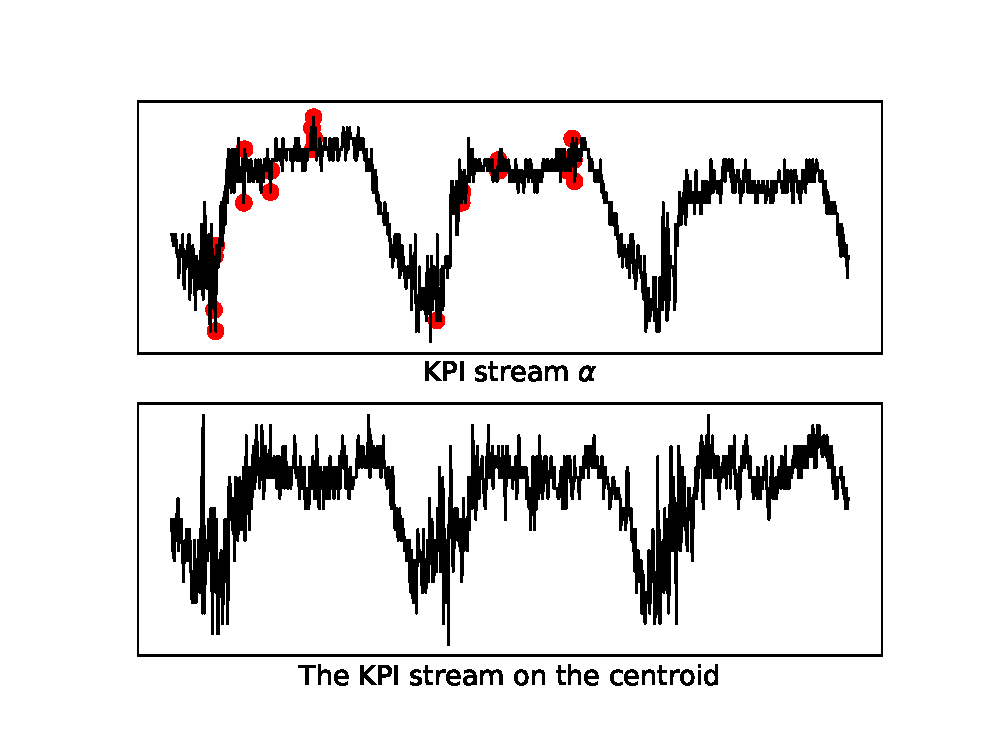
\includegraphics[width=0.9\textwidth]{fig/kpi_evaluation.eps}\\
      \end{minipage}
      %\vspace{-5 mm}
      \caption{The anomaly detection results of ROCKA + Opprentice on KPI stream $\alpha$, and $\alpha$'s cluster centroid KPI stream.
      The red data points are anomalous determined by ROCKA + Opprentice while in actual they are normal.
      }
      \label{fig:centroid_and_curve}
      \vspace{-6 mm}
     % \vspace{-1 mm}
\end{figure}

Here we explain why \name{} performs better than ROCKA + Opprentice.
KPI stream clustering methods such as ROCKA usually extract baselines (namely underlying shapes) from KPI streams and ignore fluctuations.
% The main reason is that, in order to calculate distance, ROCKA ignore the fluctuations and uses moving average to extract underlying shape of each KPI stream called baseline which will be taken as input to clustering algorithm. 
However, the fluctuations of KPI streams can impact anomaly detection.
% But the fluctuations count much in anomaly detection. 
For example, Figure~\ref{fig:centroid_and_curve} shows the new KPI stream $\alpha$, and the KPI stream on the its cluster centroid.
KPI stream $\alpha$ and the centroid KPI stream have very similar baselines, but they have different fluctuation degrees, which is not uncommon in practice.
This lead to that ROCKA + Opprentice, which is trained based only on the centroid KPI stream, generates a lot of false alarms.
% one curve 5-69 belonging to A cluster and it's centroid, the Opprentice result on it is 0.94, the \name{} results on it is 0.86, while the ROCKA+Opprentice on it is only 0.62. 
% 5-69 and it's centroid have similar baseline but vary by their fluctuations severity levels which is very common in reality. 
% Under this circumstance, the model trained by only centroid performs extremely bad. We can see that ROCKA+Opprentice determines too many normal points as anomaly points which reduces the precision.

\name{} addresses the above problem effectively using semi-supervised learning. 
In other words, it learns not only from the labels of the centroid KPI stream, but also from the fluctuation degree of the new KPI stream.
This is consistent with the observation that the model trained based on both labeled and unlabeled data should not be worse than the one trained based only on the labeled data~\cite{loog2016contrastive}.

The experiment results strongly demonstrate \name{}'s robustness in KPI anomaly detection.
% First, we get the initial model on the labelled centroid. Then, in the process of training, the model is constantly adapting to the KPI stream until finish training. 
% It not only utilizes the label information on the centroid, but also the fluctuation severity level on the KPI stream to get a satisfactory result. 
% CPLE guaranteed that . 
% If the KPI stream and it's centroid vary by their fluctuations severity levels, CPLE will continuously train to improve performance, if not, CPLE will converge very quickly and also performs well. 


% \begin{figure}
%   \begin{subfigure}[t]{0.5\columnwidth}
%     \centering
%     \includegraphics[width=.9\linewidth,height=28mm]{fig/medios.png}
%   \vspace{0.2em}
%     \caption{The centroid of cluster A}\label{fig:centroid}
%   \end{subfigure}\hfill
%   \begin{subfigure}[t]{0.5\columnwidth}
%     \centering
%     \includegraphics[width=.9\linewidth,height=28mm]{fig/5_69.png}
%   \vspace{0.2em}
%     \caption{The detection results of one curve belonging to cluster A with ROCKA+Opprentice}\label{fig:5_69}
%   \end{subfigure}
%   \caption{The detection results of one curve with ROCKA+Opprentice and it's centroid. The rea lines are anomaly points determined by the algorithm, but normal points in reality.
%   }
%   \label{fig:centroid_and_curve}
%     % \vspace{-1.2em}
% \end{figure}



% \subsection{Evaluation of aThld}
% \label{subsec:choose_threshold}
% % As of now, we have demonstrated the advantages of \name{} using best F-score in detail.
%  % However, for our system can be applied in practice, we also need to choose a the appropriate threshold from train data. 
%  % Only the point whose anomaly score given by \name{} exceeds the threshold will be regard as an anomaly point. 
%  As aforementioned, we tune aThld based on the labeling information of the testing set in order to calculate the best F-score.
%  However, it is infeasible in practice, because we cannot label the new testing set, \emph{i.e.,} the newly emerging KPI streams.
%  As discussed in Section~\ref{subsubsec:choose_threshold}, aThld can be set based on either the F-score of the labeled KPI stream (labeled-aThld henceforth), or the elbow point of the unlabeled one (unlabeled-aThld henceforth).
%  Here we compare the performance of the above two methods using the following settings.
%  % We measure the best F-score of \name{} and compared it with two ways to choose threshold as described earlier in Section~\ref{subsubsec:choose_threshold}.
% \begin{itemize}
%   \item \textbf{Labeled-aThld}. 
%   For each of the new 81 KPI streams, we set its aThld as the one that maximizes the F-score of the centroid KPI stream of the cluster where this new KPI stream belongs.
%   % We choose the threshold which maximizes the F-score on the labeled data of train.
%   \item \textbf{Unlabeled-aThld}. 
%   For each new KPI stream, we tune its aThld using the elbow point of CDF curve of the front 60\% data points' severity of this KPI stream.
%   % We choose the threshold by Elbow Point on the unlabelled data of train.
% \end{itemize}

% \begin{figure}
%       \begin{minipage}[h]{1.0\linewidth}
%       \centering
%       \includegraphics[width=0.9\textwidth]{fig/choose_thre.pdf}\\
%       \end{minipage}
%       %\vspace{-5 mm}
%       \caption{CDFs of the F-scores using labeled-aThld and unlabeled-aThld, respectively.
%       }
%       \label{fig:chooose_threshold}
%      % \vspace
% \end{figure}

% Figure~\ref{fig:chooose_threshold} shows the CDFs of the F-scores using labeled-aThld and unlabeled-aThld for 81 new KPI streams, respectively.
% Using labeled-aThld as the threshold tuning method achieves an average F-score of 0.84, which is much better than using unlabeled-aThld (the average F-score is 0.69).
% Therefore, we choose label-aThld rather than unlabeled-aThld to tune threshold for \name{}.
% Based on an on-site investigation, operators are quite satisfactory with the result achieved by label-aThld.


% Figure~\ref{fig:chooose_threshold} shows experiments' results. The average of best F-score of \name{} is 0.92, the E1 gets average 0.84 F-score, while the E2 gets only average 0.69 F-score. 
% We can determine the conclusion that E1 is the most suitable methods to choose threshold in \name{}. With the label information, E1 can find the right threshold more easily. In addtion, the experiments indicate that \name{} is of high practical value, and can be applied in real online detection with average F-score 0.84.
% {-1 mm}
% \section{Related Work}
\label{sec:related}
In this section, we will introduce recent work related to \name{} in three aspects. The first aspect is to introduce the research related to KPI anomaly detection algorithms (Section~\ref{subsec:KPI anomaly detection algorithms}). The second aspect is to introduce PU learning methods(Section~\ref{subsec:pu}). And the final aspect is an introduction to work related to active learning methods (Section~\ref{subsec:active}).

\subsection{KPI Anomaly Detection Algorithms}
\label{subsec:KPI anomaly detection algorithms}
Anomaly detection on the KPI streams refers to identifying unexpected data points from normal behavior. Over the years, lots of studies on anomaly detection for time series have been proposed. The algorithms can be divided into supervised learning methods, unsupervised learning methods, and semi-supervised learning methods.

\subsubsection{Supervised Learning Methods}
Supervised learning methods need operators' manual labels of KPI anomalies to learn algorithm selection and parameter tuning. To name some representative, EGADS~\cite{egads} separates forecasting, anomaly detection, and alerting into three separate components and uses AdaBoost~\cite{freund1997decision} to select the most relevant anomalous data points. Opprentice~\cite{liu2015opprentice} ensembles 14 widely-used traditional statistical algorithms with 133 enumerated configurations of hyper-parameters for these algorithms to extract features for the points. Then it trains a classifier using Random Forest. However, manually labeling anomalies for millions of KPI streams is not feasible.

\subsubsection{Unsupervised Learning Methods}
Unsupervised learning has emerged as a promising field in KPI anomaly detection, which does not require manual labeling. Isolation Forest~\cite{ding2013anomaly} assumes that the anomalous data points are few and different, then constructs tree structure to separate the points from the rest of points until all are isolated. The points closer to the root of the tree will be regarded as anomaly points.
Donut~\cite{xu2018unsupervised}, which is based on VAE, a deep bayesian model performs superior in accuracy. This method focuses on normal patterns instead of anomalies and tries to learn the probability distribution of the normal data points. Some other unsupervised based methods, such as Buzz~\cite{chen2019unsupervised} and Bagel~\cite{li2018robust} like Donut are also based on unsupervised learning methods to detect anomalies.

\subsubsection{Semi-supervised Learning Methods}
Semi-supervised learning~\cite{zhou2014semi} is halfway between supervised and unsupervised learning. These methods use unlabelled data to modify either parameters or models obtained from labeled data alone to maximize the learning performance of the models. ~\cite{Malhotra2015LongST} used stacked LSTM networks trained on non-anomalous data as a predictor to detect anomaly in time series. ~\cite{HighDimensional} used a combination of an one-class SVM model and a deep learning model to detect anomaly. ADS~\cite{ADSarticle} used clustering and CPLE~\cite{loog2016contrastive} to detect anomaly in time series. Although semi-supervised learning based methods do reduce the cost of manually labeling, it is very difficult for operators to label all the anomalous data points in those specified time series segments and ensure accuracy.

\subsection{PU Learning Methods}
\label{subsec:pu}
PU learning is suitable for lots of applications in text detection~\cite{Li2014SpottingFR, Liu2002PartiallySC, putranditional2003, ren-etal-2014-positive} and  bioscience~\cite{Mordelet_2011, Yang2014EnsemblePU}. ~\cite{putranditional2003}firstly regarded the unlabeled samples as negative samples and used a spy technique to introduce some positive instances to mixed sets and then got the threshold score between positive and negative classes.  ~\cite{Liu2002PartiallySC}proposed a technique which combines the Rocchio method and the SVM technique for classifier building, while the first step is also treating all unlabeled samples as negative set. 
It is not feasible to assume that all unlabeled samples are negative samples, because most of the training data in time series anomaly detection is positive. ~\cite{PUlearning2017} improved previous PU learning methods so that it could apply for time series anomaly detection and made it suitable for the unbalanced scenario. In our \name{}, we utilize the PU learning based~\cite{PUlearning2017} to label abnormalities as few as possible and achieve better results than the semi-supervised learning methods.

\subsection{Active Learning}
\label{subsec:active}
In \name{}, active learning is used to label unlabeled samples, thereby helping the PU learning algorithm to obtain more reliable normal samples. ~\cite{Outlieractive}used a selection strategy based on active learning to reduce the classification problem of anomaly detection. ~\cite{Pelleg04activelearning}proposed a novel active learning method to identify rare category records in an unlabelled noisy set with a small budget of data points that they are prepared to categorize. Most of the active learning methods such as~\cite{activelearning2015} selected samples on the classification boundary to label, while via experiments in our KPI streams, choosing the unlabeled data likely to be normal to label is the best selection strategy which is more suitable for KPI streams data.
%!TEX root = ../cluster_semi.tex
\section{Conclusion}
\label{sec:conclusion}

 To the best of our knowledge, this paper is the first to identify the common and important problem of \textit{rapid deployment of anomaly detection models for large number of emerging KPI streams, without manual algorithm selection, parameter tuning, or new anomaly labeling for any newly generated KPI streams}. We propose the first framework \name{} that tackles this problem via clustering and semi-supervised learning, which is the first time that semi-supervised learning is applied to KPI anomaly detection. 
 Our extensive experiments using real-world data show that, with the labels of only the 5 cluster centroids of 70 historical KPI streams, \name~achieves an averaged best F-score of 0.92 on 81 new KPI streams, almost the same as the state-of-art supervised approach~\cite{liu2015opprentice}, and greatly outperforms an unsupervised approach Isolation Forest~\cite{zhang2018anomaly} by 360\% and the state-of-art unsupervised approach Donut~\cite{xu2018unsupervised} by 61.40\% on average.  
     
We believe that \name{} is a significant step towards practical anomaly detection on large-scale KPI streams in Internet-based services. In the future, we plan to adopt more advanced techniques (\EG{} transfer learning~\cite{pan2010survey}) to further improve \name{}'s performance.

%\section{acknowledgements}
\label{acknowledgements}
We thank Shuai Yang, Tianheng Zuo for their helpful suggestions.
The work was supported by National Natural Science Foundation of China (NSFC) under grant No. 61402257, No. 61472214, No. 61472210 and No. 61772307, and Tsinghua-Tencent Joint Laboratory for Internet Innovation Technology.


\bibliography{IEEEabrv,references}
\bibliographystyle{IEEEtran}


\end{document}
